\documentclass[10pt,a4paper]{article}
\usepackage{times}
\usepackage{ctex}  
\usepackage{color}   

\usepackage{listings}
\usepackage[usenames,dvipsnames]{xcolor}
\definecolor{mygreen}{rgb}{0,0.6,0}
\definecolor{mygray}{rgb}{0.5,0.5,0.5}
\definecolor{mymauve}{rgb}{0.58,0,0.82}
\lstset{
 backgroundcolor=\color{lightgray}, 
 basicstyle = \footnotesize,       
 breakatwhitespace = false,        
 breaklines = true,                 
 captionpos = b,                    
 commentstyle = \color{mygreen}\bfseries,
 extendedchars = false,             
 frame =shadowbox, 
 framerule=0.5pt,
 keepspaces=true,
 keywordstyle=\color{blue}\bfseries, % keyword style
 language = C++,                     % the language of code
 otherkeywords={string}, 
 numbers=left, 
 numbersep=5pt,
 numberstyle=\tiny\color{mygray},
 rulecolor=\color{black},         
 showspaces=false,  
 showstringspaces=false, 
 showtabs=false,    
 stepnumber=1,         
 stringstyle=\color{mymauve},        % string literal style
 tabsize=2,          
 title=\lstname                      
}

\usepackage{comment}
\usepackage{amsmath}
\usepackage{amssymb}
\usepackage{amsthm}
\usepackage{amscd}
\usepackage{graphicx}
\usepackage{subfigure}
\usepackage{indentfirst}
\usepackage{titlesec}
\usepackage{url}
\usepackage[top=25.4mm, bottom=25.4mm, left=31.7mm, right=32.2mm]{geometry}


\newtheoremstyle{mythm}{1ex}{1ex}
{\songti}{\parindent}{\heiti \bf}{}{1em}{}
\theoremstyle{mythm}
\newtheorem{thm}{定理~}[section]
\newtheorem{lem}[thm]{引理~}
\newtheorem{pro}[thm]{性质~}
\newtheorem{fact}[thm]{Fact}
\newtheorem{prop}[thm]{命题~}
\newtheorem{ques}[thm]{问题~}
\newtheorem{cor}[thm]{推论~}
\newtheorem{de}[thm]{定义~}
\newtheorem{rem}[thm]{注记~}
\numberwithin{equation}{section}

\renewcommand\refname{\heiti 参考文献}

\makeatletter
\renewenvironment{proof}[1][\proofname]{\par
\pushQED{\qed}%
\normalfont \topsep6\p@\@plus6\p@ \labelsep1em\relax
\trivlist
\item[\hskip\labelsep\indent
\bfseries #1]\ignorespaces
}{%
\popQED\endtrivlist\@endpefalse
}
\makeatother

\renewcommand{\proofname}{\heiti 证明}

\renewcommand{\thefootnote}{\fnsymbol{footnote}}

\titleformat{\section}{\large \bf \heiti }{{\bf \thesection\space}}{0pt}{}

\begin{document}

\setlength{\abovedisplayskip}{1ex}
\setlength{\belowdisplayskip}{1ex}

\author{胡星宇 (21921150)}    
\title{TEB复现 
Trajectory modification considering dynamic constraints
of autonomous robots}           
\maketitle                                          
\section{1.引言}
这篇文章是对TEB算法的复现,这一次准备记录整个算法和ros\_ teb\_ planner的学习过程,逐渐完善本篇。对论文的原理不在本文中介绍,相关的资料网上有。但是网上的资料其实说的很不清楚。因此下面我会按照以下顺序结构进行本文的完成:

在第二节中主要是对方法的介绍,2.1节是理解了的方法,2.2节是没理解的问题。

在第三节中尝试绘制算法流程图,并对比ros源代码逐渐修改。3.1节是计算的流程。3.2节是流程每部分对比ros。3.3节是一些代码思考和改进点。3.4节是问题记录。

在第四节中主要是数据结构的完成,主要实现的功能以及类的关系等。

在第五节中主要学习g2o优化库的写法,因为之前比较熟悉的是ceres,这次使用g2o进行优化。5.1节是g20,5.2节是与ceres的对比。

第六节是代码复现中遇到的问题记录。
\section{2.方法概述}
\subsection{2.1已理解部分}
TEB主要是对局部路径点的优化,每个点都有很多约束,它求解的是带约束条件的最小二乘问题。论文中提到了很多约束,这里我理解的约束有:

1.与全局路径点的距离或者障碍物距离的约束。这个约束定义为:

\begin{equation}
e_{\Gamma}(x,x_{\gamma},\epsilon,S,n)\simeq
\left\{
             \begin{array}{lr}
             \frac{(x-(x_\gamma - \epsilon))}{S}^n & if \quad x > x_{\gamma} - \epsilon \\
             0 & otherwise  
             \end{array}
\right.
\label{eq:constrain_distance}
\end{equation}
这个约束的意思就是超过规定的距离,函数值就越大,$x$指局部点与全局路径点或者障碍物点的最小距离,$x_{\gamma}$指设定的最大半径,$\epsilon$表示这种计算的扰动近似,主要是避免浮点运算的。对这个函数最小化,就是要求实际运动的点尽量靠近全局点,但也要尽量远离障碍物(障碍物其实就是把距离和半径都取负数)。

2.速度和角速度的计算,公式如下:
\begin{equation}
v_i \simeq \frac{1}{\Delta T_i}\|\left(
\begin{array}{lr}
x_{i+1}-x_i\\
y_{i+1}-y_i
\end{array}
\right)
\|
\label{eq:velocity}
\end{equation}

\begin{equation}
w_i \simeq \frac{\beta_{i+1}-\beta_i}{\Delta T_i}
\label{eq:rad}
\end{equation}

另外加速度是通过两点间速度计算的:
\begin{equation}
\alpha_i =  \frac{2(v_{i+1}-v_i)}{\Delta T_i+\Delta T_{i+1}}
\label{eq:accelerate}
\end{equation}

注意到这里速度,角速度,加速度都有自己的限制,这是车辆或者用户设定的,而这三个值都与$\Delta T$有关,也就是时间,事实上,我们的目标是最快抵达目的地,所以$\Delta T$要尽量少,也就是在满足上述三个方程在人为给定的限制内,使$\Delta T$尽量小。所以上面三个方程是约束条件。

3.相邻点的约束。
\begin{figure}[htbp]
\centering  %图片全局居中
\label{Fig.main}
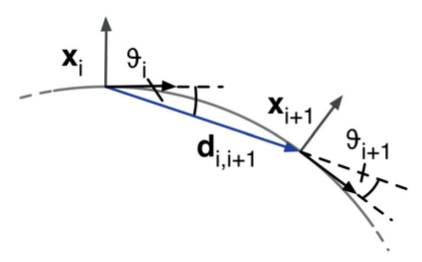
\includegraphics[width=0.45\textwidth]{TEB_1}
\caption{运动约束}
\end{figure}
论文中考虑的是速度差分运动的机器,husky也属于这类,这类运动满足当角速度不变是进行圆弧运动。于是作者假设两个局部点间的角速度不变。那么两点间的向量和两个点处机器人的朝向($\beta_i$和$\beta_{i+1}$)满足如下关系:
\begin{equation}
\theta_i =  \theta_{i+1}
\label{eq:theta_equal}
\end{equation}

\begin{equation}
\left(
	\begin{array}{lr}
	cos\beta_i\\
	sin\beta_i\\
	0\end{array}
\right)\times d_{i,i+1} = d_{i,i+1}\times
\left(
	\begin{array}{lr}
	cos\beta_{i+1}\\
	sin\beta_{i+1}\\
	0\end{array}
\right)
\label{eq:sinTheta_equal}
\end{equation}
注意向量叉乘有个性质就是交换一下正好就是负数,所以这里可以写成:
$$
\left(
	\begin{array}{lr}
	cos\beta_i+cos\beta_{i+1}\\
	sin\beta_i+sin\beta_{i+1}\\
	0\end{array}
\right)\times d_{i,i+1} = 0
$$

于是构造如下函数:
\begin{equation}
f_k(x_i,x_{i+1})=\left\|
\left(
	\begin{array}{lr}
	cos\beta_i+cos\beta_{i+1}\\
	sin\beta_i+sin\beta_{i+1}\\
	0\end{array}
\right)\times d_{i,i+1}\right\|^2
\label{eq:point_constrain}
\end{equation}

对这个函数最小化等价于尽量去满足速度差分的运动学约束。
最后一个最小化的目标就是
$$
f_k=\left(\sum_{i=1}^{n}\Delta T_i\right)^2
$$

这就是追求最快抵达目标的函数。
\subsection{2.2未理解部分}
1.这些局部点是怎么划分的?

关于这个问题,ros代码中有一段说明是:所实现的算法使用给定的离散宽度对开始和目标之间的直线进行二次采样。 可以使用diststep参数在欧几里得空间中定义离散宽度。 两个连续姿势之间的每个时间差都会初始化为时间步长。 如果将diststep选择为零,则生成的轨迹仅包含起点和目标姿势。

可以发现这种划分是需要人为设定的。

另外还有一种初始化方法:从通用2D参考路径初始化轨迹。 使用给定的最大速度(包含平移和角速度的2D矢量)确定时间信息。 实现了恒定速度曲线。 如果提供max\_ acceleration参数,则考虑可能的最大加速度。 由于方向未包含在参考路径中,因此可以单独提供(例如,根据机器人姿势和机器人目标)。 否则,目标标题将用作开始和目标方向。 沿着轨迹的方向将使用参考路径的两个连续位置之间的连接矢量来确定。

可以看到,另一种方法依赖全局路径得到的。这两种方法都在同名函数initTrajectoryToGoal中(一共有三个,不过后两个似乎差不多)。我们先分析第一种方法的实现过程:
1)把起点加入到vector中并设置为不可变点。
2)初始化时间间隔为0.1,计算起点和终点的向量,计算每步长在x方向和y方向的投影(dx,dy),计算初始朝向,如果终点在起点身后,朝向要旋转180°,如果设置了最大速度,计算时间步长=距离/速度。
3)通过计算的步长和时间间隔,把起点到终点的直线分割成许多局部点,放入vector中待优化。把时间间隔也插入到difftime的vector中
4)如果分割的点小于要求的最小数量,就需要再在中间插入一些点,直到满足数量要求。
5)最后把目标点插入进去作为最后一个点

第二种方法是已经获得了全局规划的点:
1)插入起点
2)对全局规划的每个点,如果没有提供pose,计算两点间pose,然后插入该点
3)如果数量不够,再多插入一些
4)插入终点

2.为什么速度差分在角速度不变时是圆弧?

网上直接默认的就是圆弧运动。其旋转半径为
$$
R = \frac{l}{2}\frac{v_r+v_l}{v_r-v_l}
$$ 

3.论文提到如果是角度变化180°,需要特殊处理,如何处理?

代码里的办法是如果角度在这个pose的身后,那么计算出来的pose需要加$\pi$。

\section{算法流程}
\subsection{流程图}
\begin{figure}[htbp]
\centering  %图片全局居中
\label{Fig.2}
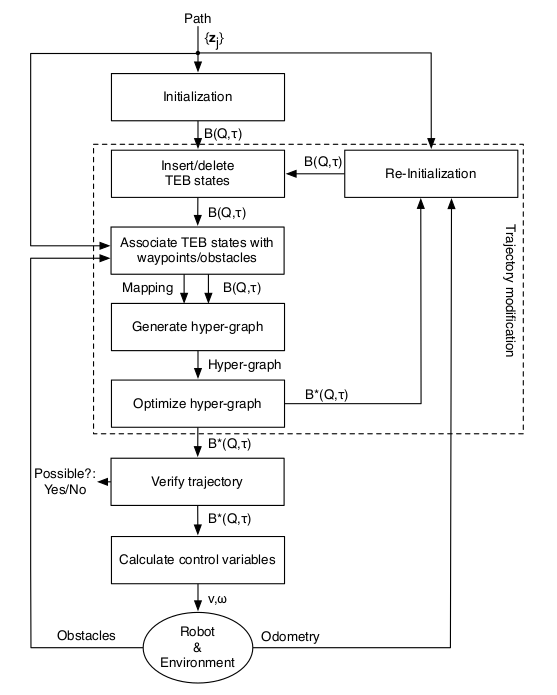
\includegraphics[width=1\textwidth]{teb_flow}
\caption{算法流程图}
\end{figure}
论文中的算法流程见图\ref{Fig.2}。
前两步在上一节中已经介绍过。接下来看看如何将局部点和路径点与障碍物点联系起来。
\subsection{ros中的处理过程}
约束的公式在前面已经介绍过了,但问题是给定的全局点以及障碍物点到底与哪个局部点构成了约束?
寻找与一个局部点最近的点的约束在代码中是一系列同名函数:
findClosestTrajectoryPose。
针对点,线,多边形以及障碍物类型来计算最近的约束条件。
先看点与点间如何计算的。

点与点的计算非常简单,遍历所有的局部点,找到与参考点欧式距离最近的点即可。

点与参考线的计算其实就是计算点与线段间的距离,遍历所有局部点,选取最近的即可。

点与多边形的计算是点与多条线段的距离的最小值。

最后一个其实是汇总,根据障碍物类型来计算,对于不属于上述类型的障碍物,取中心点进行点计算。

有了每个局部点与相关联点的联系,就可以构造约束了。

现在的问题是增加哪些点和局部点的联系?
在AddEdgesObstaclesLegacy函数中,我们可以看到,逻辑是设置一个影响点的个数n,然后对于所有的障碍物点,通过findClosestTrajectoryPose寻找最近点,并对附近$±\frac{n}{2}$个点也添加约束。添加约束在g2o中是增加边,具体操作后续在g2o中再分析。

障碍物可以分成静止的障碍物和动态的障碍物,对静止障碍物用上面方法就可以了,但动态的是在AddEdgesDynamicObstacles中处理。动态障碍物的约束论文里没提,这是一个问题。

现在的问题是障碍物如何添加到planner中?
这里teb\_ planner提供两种方法,一种是通过costmap\_ convert将costmap转换成二维的线,多边形等进行处理。另一种是不通过costmap\_ convert,把所有的障碍物的点都视作点来处理。

梳理一下现在的流程:
1.通过costmap获得局部地图上的障碍物的点。通过global\_ planner获得全局路径。
2.每次需要计算速度和角速度时,就截取全局路径的一部分,同时更新一次costmap的信息获取obstacle的点。
3.调用plan函数。对截取的全局路径进行划分,得到局部点,遍历局部点计算有影响的障碍物点,并进行一定范围的扩展,然后把这些影响都放入g2o的边中。
4.开始优化:优化过程分为两个循环,外循环每次需要调整点的间隔,时间间隔太大就划分一个新的点,太小就删除。修改完毕后开始建立优化图。优化图的顶点是局部点的位置和朝向,边是各种约束,约束的公式是放在继承的g2o::BaseUnaryEdge类里重写的。需要特别说明一下,速度,角速度,加速度这类有范围的用的是\ref{eq:limit1}和\ref{eq:limit2}:
\begin{equation}
f(x,limit,\epsilon) = 
\left\{
             \begin{array}{lr}
             0 \quad if \quad \|x\|\leq limit\\
             \|x-(limit-\epsilon)\| \quad otherwise  
             \end{array}
\right.
\label{eq:limit1}
\end{equation}
\begin{equation}
f(x,lower,upper,\epsilon) = 
\left\{
             \begin{array}{lr}
             lower+\epsilon-x \quad if \quad x < lower+\epsilon\\
             0 \quad lower+\epsilon \leq x\leq upper-\epsilon\\
             x-(upper-\epsilon) \quad if \quad x > upper-\epsilon  
             \end{array}
\right.
\label{eq:limit2}
\end{equation}
这类公式有很多变化,总之就是在要求的范围内为0,超出范围就开始根据连续性进行惩罚。

建立图后就可以开始通过g2o优化

另外还有一个细节是车辆的footprint,我们不能把车辆当成一个点,所以这个
也是要处理的,不过这个在ros的cosmap中已经提供方法了,就是costmap\_ 
2d::calculateMinAndMaxDistances,能计算footprint的最大半径和最
小半径。
\subsection{思考与改进}
可以看到teb没有对动态障碍物的躲避,事实上,移动物体的避障,用传统的计算方法很难进行,因为要预测所有移动物体的轨迹。光流法可以定位移动物体。问题在于如何对移动物体进行约束。运动学公式是什么?能解决这个问题,才能解决teb的优化算法对运动物体的计算。
\subsection{待处理问题}
1.动态障碍物的约束公式是什么?
这个在teb中实际是没有处理的,这是一个研究点。

2.车辆的footprint如何处理的?
通过costmap提供的函数将footprint转换为maxradius和minradius。

3.优化的外循环中有个权重算子weight\_ multiplier,每次外循环就累乘一
个weight\_ adapt\_ factor,目的?


\section{数据结构}
分析一下需要处理的东西。我们需要一个配置类来收集所有的配置数据。暂定为configuration类。配置数据信息在子节中列出。
需要一个类来接受输入,比如path信息,并进行初始化,它保存了所有的局部点和时间间隔,并且能根据地图信息进行处理。这个类是与ros通信的接口类,可以叫做teb\_ ros类。planner类是用来核心处理整个局部路径计算的。

然后在planner类中有一个优化器类optimizer,这个类是teb与g2o的接口。

其他还需要的是一些定义g2o优化函数的类。这些类都继承自g2o的点和边。
一些辅助函数放在utils类中。
\subsection{configuration类}
配置中分为几类配置,trajectory相关,robot相关,goal相关,obstacle相关,optimization相关,Homotopy和Recovery的参数没搞明白用法,这里也列出来,后续仔细分析。
\subsubsection{trajectory}
策略中主要包括局部点的时间分辨率的自动调整大小(teb\_ autosize),期望的时间分辨率(dt\_ ref),迟滞的变化率(dt\_ hysteresis)(就是向着期望值逼近的快慢速度),最大最小采样数(min\_ samples,max\_ samples),是否允许全局路径的朝向覆盖局部路径的朝向,是否允许向后运动的初始化,是否按照给出的全局点安排局部点的顺序,最大的规划点数量(max\_ global\_ plan\_ lookahead\_ dist),在出现新目标时是否完全重新计算,需要检查可行性pose的数量(feasibility\_ check\_ no\_ poses),是否发布反馈,碰撞检测的最小角度分辨率,计算速度所需的点(control\_ look\_ ahead\_ poses)
\begin{lstlisting}[caption={trajectory结构体}]
struct Trajectory
{
  double teb_autosize;
  double dt_ref;
  double dt_hysteresis;
  int min_samples;
  int max_samples;
  bool global_plan_overwrite_orientation;
  bool allow_init_with_backwards_motion;
  double global_plan_viapoint_sep;
  bool via_points_ordered;
  double max_global_plan_lookahead_dist;
  double global_plan_prune_distance;
  bool exact_arc_length;
  double force_reinit_new_goal_dist;
  double force_reinit_new_goal_angular;
  int feasibility_check_no_poses;
  bool publish_feedback;
  double min_resolution_collision_check_angular;
  int control_look_ahead_poses;
}
\end{lstlisting}
\subsubsection{robot}
关于robot的参数,主要是运动性能的约束,最大速度,最大后退速度,最大切向速度,最大速度角,最大加速度,最大切向加速度,最大角加速度,最小旋转半径,对于速度差分机器最小旋转半径是0,当然汽车这类的旋转半径是和轴距以及轮子的最大转角有关的。
\begin{lstlisting}[caption={robot结构体}]
struct Robot
{
  double max_vel_x;
  double max_vel_x_backwards;
  double max_vel_y;
  double max_vel_theta;
  double acc_lim_x;
  double acc_lim_y;
  double acc_lim_theta;
  double min_turning_radius;
  double wheelbase;
  bool cmd_angle_instead_rotvel;
  bool is_footprint_dynamic;
  bool use_proportional_saturation;
}
\end{lstlisting}
\subsubsection{goal}
关于goal的参数,主要是判断抵达goal的依据,比如与目标要求的pose之间的偏差最大在多少,与目标坐标的距离最大在多少时认为抵达目标点,是否允许带速抵达目标,是否不允许以经过目标的方式抵达目标。
\begin{lstlisting}[caption={goal结构体}]
struct Goal
{
  double yaw_goal_tolerance;
  double xy_goal_tolerance;
  bool free_goal_vel;
  bool complete_global_plan;
}
\end{lstlisting}
\subsubsection{obstacle}
包括与障碍物的最小距离,膨胀距离(就是说这个距离可以抵达,但是要受到惩罚),动态障碍膨胀距离(不知道实现了没有),是否考虑动态障碍物,是否包括costmap中的障碍物,受障碍物影响的局部点个数,是否使用传统的障碍物关联算法(传统算法是对每个障碍物,找局部点,其他的算法还有通过局部点寻找影响点的障碍物),非传统算法考虑障碍物的半径系数,非传统算法中优化过程忽略障碍物的半径系数(超过某个值的距离就在优化时忽略),costmap\_ convert插件名(costmap\_ convert可以把costmap上的障碍物转换成line或者多边形之类的,需要设置转换的插件名),costmap\_ convert的线程数,转换率,遇到障碍物的最大减速,需要减速的距离和需要加速的距离,
\begin{lstlisting}[caption={Obstacles结构体}]
struct Obstacles
{
  double min_obstacle_dist; 
  double inflation_dist;
  double dynamic_obstacle_inflation_dist;
  bool include_dynamic_obstacles;
  bool include_costmap_obstacles;
  double costmap_obstacles_behind_robot_dist;
  int obstacle_poses_affected;
  bool legacy_obstacle_association;
  double obstacle_association_force_inclusion_factor;
  double obstacle_association_cutoff_factor;
  std::string costmap_converter_plugin;
  bool costmap_converter_spin_thread;
  int costmap_converter_rate;
  double obstacle_proximity_ratio_max_vel;
  double obstacle_proximity_lower_bound;
  double obstacle_proximity_upper_bound;
}
\end{lstlisting}
\subsubsection{optimization}
优化参数有内部循环次数,外部循环次数,是否激活优化,是否打印详细信息,惩罚系数$\epsilon$,对限制参数的权重设置(这些权重主要是用来衡量各个约束的重要性程度的),非线性障碍物的指数(一般为1,即不考虑非线性)。

\begin{lstlisting}[caption={Optimization结构体}]
struct Optimization
{
  int no_inner_iterations; 
  int no_outer_iterations;
  bool optimization_activate;
  bool optimization_verbose;
  double penalty_epsilon;
  double weight_max_vel_x;
  double weight_max_vel_y;
  double weight_max_vel_theta;
  double weight_acc_lim_x;
  double weight_acc_lim_y;
  double weight_acc_lim_theta;
  double weight_kinematics_nh;
  double weight_kinematics_forward_drive;
  double weight_kinematics_turning_radius;
  double weight_optimaltime;
  double weight_shortest_path;
  double weight_obstacle;
  double weight_inflation;
  double weight_dynamic_obstacle;
  double weight_dynamic_obstacle_inflation;
  double weight_velocity_obstacle_ratio;
  double weight_viapoint;
  double weight_prefer_rotdir;
  double weight_adapt_factor;
  double obstacle_cost_exponent;
}
\end{lstlisting}
剩下两个结构体应该是用来计算多条局部路线和遇到一些问题的恢复方法参数。目前还没有详细分析,待完善。
\subsection{teb\_ ros类}
teb\_ ros类是用来在ros中通信的,它应当是接口,用来处理ros的输入,比如全局路径规划传递的path等。

它具备的功能如下:

1.接受全局路径规划的plan消息,保存此plan用于teb处理。

2.处理全局plan,把不适合的部分裁剪掉。

3.对teb处理得到的当前速度和角速度指令,向cmd\_ vel发布消息。

4.判断经过teb控制的无人车是否已经抵达目的地。

5.取消teb的控制指令

6.读取用户给出的footprint信息,并进行转换。

7.从param中获取配置信息,并传递给configuration类。

\subsubsection{成员变量}
该类需要接受teb处理的输入信息,以及发送输出信息,由于它是接口类,所以成员函数包括以下几类:

1.teb类指针

2.configuration类指针

3.costmap类指针

4.障碍物信息

5.全局路径信息

6.位姿信息

7.目标位姿

8.footprint信息
\subsubsection{消息订阅与发布}
可以看到,该类至少需要plan消息,obstacle消息,costmap可以从move\_ base传递指针过来,不需要消息传递。发布的消息,ros\_ teb源码的做法是用move\_ base去调用ros\_ teb中的函数,再在move\_ base中发布,这里为了保持插件的统一,也采取这种做法。

代码中真正订阅的消息非常少,大部分需要的输入都是从move\_ base中调用函
数传递数据进来的。
\subsubsection{初始化}
需要注意,teb\_ ros是ros的局部路径规划器的接口类,所以必须满足接口函数,为了满足此要求,teb\_ ros是继承nav\_ core::BaseLocalPlanner和 mbf\_ costmap\_ core::CostmapController的。初始化过程需要为costmap、teb\_ planner、configuration等赋值,对接口类进行初始化赋值,核心操作其实是从move\_ base获取到了costmap,global\_ plan的指针,用来方便进行局部路径规划。
\subsubsection{重载函数}
nav\_ core::BaseLocalPlanner是虚类,拥有以下函数需要重载:
\begin{lstlisting}[caption={BaseLocalPlanner}]
virtual bool computeVelocityCommands (geometry_msgs::Twist &cmd_vel)
virtual void initialize (std::string name, tf::TransformListener *tf, costmap_2d::Costmap2DROS *costmap_ros)
virtual bool 	isGoalReached ()
virtual bool 	setPlan (const std::vector< geometry_msgs::PoseStamped > &plan)
virtual 	~BaseLocalPlanner ()
\end{lstlisting}
mbf\_ costmap\_ core::CostmapController多一个cancel()函数,其余都一样。
因此这几个函数是必须实现的,从这几个函数也可以看到,在initialize中输入了tf树,costmap指针,而全局路径规划的plan是通过setPlan传递的。
\subsubsection{辅助函数}
一些其他功能在类功能描述中已经提到了。这里需要重点提一个,就是拥有costmap指针后,需要用一种数据结构或者存储方式来实时更新障碍物信息,如果没有costmap\_ convert插件,costmap中的障碍物点都要保存下来。保存和更新的方法如下(无convert时):

遍历costmap的每个grid,如果障碍物不是在车辆身后或者离车非常近的地方(防止误差),构造障碍物点的类指针,并放入vector中。

(有convert时):

从costmap\_ convert中获取障碍物,然后根据各种属性比如点的个数和半径数值等判断这个障碍物的类别(point,line,circle,polygon等),根据类别构造不同的障碍物类,并保存其指针。

全局路径的裁剪:
全局路径的裁剪逻辑非常简单,遍历全局路径的点,如果与当前robot的位置的距离小于设定的距离,就说明这个点已经经过了,然后把从begin到这个点的所有点都erase掉。
\subsection{planner类}
planner类是通过teb\_ ros的plan调用的,其输入是global plan的路径点和当前速度,角速度,计算出一系列局部点,然后当需要得到当前点的下一步速度角速度时在通过优化完的点计算出来。它的功能包括:
1.初始化一些配置,并获取obstacle的指针以便计算约束。
2.读取全局路径,产生初始的局部点,来构造一个优化问题
3.teb\_ ros能在plan完毕后询问planner当前位姿,速度,角速度下的下一步行动。
4.能够根据局部点和配置,添加各种约束。
5.能够处理全局plan的变化。

\subsubsection{成员变量}
成员变量里面必然有configuration的指针,obstacle的指针和需要构造的优化器的类接口,另外源代码中不知道为何,planner还提供一个teb的接口,这个teb类似乎只是用来处理局部点的间隔和时间间隔这个弹簧带的,这是一个封装的数据结构,后续详细分析。
\subsubsection{初始化}
初始化需要teb\_ ros提供configuration的指针,obstacle指针,然后根据配置构造optimizer和teb类。

\subsubsection{优化流程}
首先收到plan信息后,先通过teb类构造出初始局部点和时间间隔,如果有必要,把plan中已经过时的部分裁剪去。然后开始优化。

优化的时候,首先根据初始局部点,障碍物信息,配置要求添加所有的约束,然后用optimizer创建图,调用optimizer进行图优化。

当接口询问当前速度,角速度时,从当前位置,搜索前面几个局部点的状态(数量是人为设定的),获得距离,位姿和时间,然后进行简单的计算就可以了。
\subsection{teb类}
teb类是管理时间间隔和局部点的,时间间隔和局部点都是用容器管理,同时teb类具备初始化一个弹簧带的能力,这在前面提到过,它可以根据起点和终点产生一个带,也可以通过全局路径产生。功能如下:
1.管理容器的插入,添加,删除和查询
2.初始化弹簧带
3.更新和裁剪弹簧带
4.对给定的点,寻找有影响的局部点。
\subsubsection{成员变量}
成员变量主要是两个容器,局部点容器和时间间隔容器。
\subsubsection{重要函数}
这里其他的功能前面都详细说过,主要是更新和裁剪弹簧带是如何实现的,这需要说明一下:

首先当出现一个新的plan时,产生新的起点和终点,此时原来的局部点中在新起点前面的那些优化就没用了,需要删除掉,此时的做法是从头遍历容器,把距离逐渐缩短的点记录下来,当距离增大时说明点在起点之后了,记录最后一个index,然后从1到index的局部点和时间间隔都删除,把0赋值新起点。

另外还有一个是自动调整带大小的操作:

对于时间间隔,我们既不希望时间间隔太长也不希望太短,是在一个我们设定的范围内。对于长的,就把它减半,然后分成两个间隔,pose取中间值,反正也要优化的。短的就合并,然后删除没用的那个。

\section{g2o优化库}
teb调用g2o的地方在planner里面,成员变量:

boost::shared\_ ptr<g2o::SparseOptimizer> optimizer\_ ;

optimizer使用到的函数有:

addEdge()

edges().empty() 

vertices().empty()

initializeOptimization()

computeInitialGuess()

activeEdges().begin() end()(点和边在g2o里应该是容器)

setAlgorithm()

initMultiThreading()

setVerbose()显示优化的信息

optimize()

addVertex()

\subsection{初始化创建优化器}

初始化首先构造SparseOptimizer,然后选择线性求解方法(这里选择的是
CSparse,其实我也不确定PCG是不是好一些,不过这么大型稀疏的矩阵,应该是
CSparse好用)
然后用线性求解器来构造块求解器,再用块求解器构造求解方法。
求解方法选择的是g2o::OptimizationAlgorithmLevenberg。
最后使用optimizer->setAlgorithm(solver)和optimizer->initMultiThreading()来设置优化器的求解方法和多线程。就得到一个优化器了。

\subsection{添加点和边}
这里有必要说一下,g20由于是依靠图进行运算的,所以计算的变量是点,计算公式是边,就是有多少个方程,就有多少条边,jacobi的计算也是通过边完成的,所以需要自定义点和边,就是定义变量和约束公式。

首先看点。点就是变量,在teb中优化的变量是局部点的位姿和时间间隔。
先看局部点的定义。

局部点定义了一个包含位姿和朝向的类:

class VertexPose : public g2o::BaseVertex<3, PoseSE2 >
PoseSE2是teb自定义的位姿类,这个定义的意思是,该点的输入是PoseSE2
类,其中有3个参数可以优化。
注意,有两个函数必须要写,就是参数的重置和参数的更新,这两个函数分别为:
virtual void setToOriginImpl()和virtual void 
oplusImpl(const double* update\_ )。需要我们实现参数的重置和更
新。

还有一个函数经常用到,叫setFixed(bool),这个函数本身就提供,可以用来
关闭该点的优化。

另一个顶点的是时间间隔,显然是变量个数为1的顶点。
边的定义:
边有很多种类型,根据约束公式的定义逐渐说明。
\subsubsection{加速度约束边}
class EdgeAcceleration : public BaseTebMultiEdge<2, double>

加速度约束的公式,这个类表示有两个残差,类型是double。
它最终继承的是g2o::BaseMultiEdge,这个类有如下成员函数需要继承:
1.virtual void 	linearizeOplus ()
2.virtual void 	resize (size\_ t size)
3.computeError()
4.read()
5.write()

构造的时候用这几个就足够了,第一个是计算jacobi的,第三个是计算误差的。
加速度约束中,需要用到3个点的位姿和两个时间间隔(见公式\ref{eq:accelerate}),所以这个边连接了5个点,位姿1,位姿2,位姿3,时间间隔1,时间间隔2,有两个误差项,分别是加速度和角加速度,误差公式是采用越界惩罚的形式进行的。jacobi的计算可以自己写,也可以不写,不写的话g2o会用数值求导的方式把导数算出来(不明白teb这里为什么让g2o数值求导,因为数值求导需要计算误差值多次,还要引入小变量,比较费计算的环节)。

注意还有两个特殊的加速度约束边。因为速度是用三个位姿计算的,但在起点和终点不满足三个位姿,此时第一个速度或者第二个速度设置为起点速度或者终点速度,然后只计算剩下那个,因此点只有三个(位姿1,位姿2和时间间隔1)

\subsubsection{运动学约束边}
class EdgeKinematicsDiffDrive : public BaseTebBinaryEdge<2, double, VertexPose, VertexPose>

运动学的约束公式见公式\ref{eq:point_constrain},它只和两个局部点的位姿和朝向有关系,所以用的是BaseTebBinaryEdge,两个点的类型都是VertexPose,注意,这里的2表示残差有两个,但是从公式\ref{eq:point_constrain}上可以看出来,残差是叉积,应该只有一个。这多出来的另一个实际上是运动方向的约束,即两个点之间的方向向量和第二点的朝向要是正数,负数要受到惩罚。

\subsubsection{障碍物约束边}
class EdgeObstacle : public BaseTebUnaryEdge<1, const Obstacle*, VertexPose>

障碍物边是一元边,就是可变参数只和常数产生联系,这里的常数就是obstacle,位姿就是变量。

这里的error只有一个,就是障碍物与该局部点的距离的约束,但是需要注意的是,局部点虽然是一个点,但代表的是车辆模型,所以其实是计算相关的障碍物与footprint构造的多边形的距离。
\subsubsection{转向约束边}
class EdgePreferRotDir : public BaseTebBinaryEdge<1, double, VertexPose, VertexPose>

这也是teb上没提到的一个约束,就是如果有一个局部点有特殊的转向方向,比如左转、右转,那么就要设置一个惩罚,当违法了设定时给出截断惩罚函数。

\subsubsection{最短路径约束边}
class EdgeShortestPath : public BaseTebBinaryEdge<1, double, VertexPose, VertexPose>

最短路径约束边是两向边,就是让两个position之间的距离尽量短。

\subsubsection{时间最短约束边}
class EdgeTimeOptimal : public BaseTebUnaryEdge<1, double, VertexTimeDiff>

这个更直接,我们的变量是时间间隔,用一个一元边约束,让时间间隔尽量短。

\subsubsection{速度约束边}
class EdgeVelocity : public BaseTebMultiEdge<2, double>

这里是一个多元边,因为速度需要两个局部点和一个时间间隔共三个顶点来计算。这里速度的计算不是两个局部点的直线距离,而是计算弧长再除以时间间隔得到线速度,角速度比较好计算,是角度的变化率,然后用截断公式来得到约束。

\subsubsection{速度障碍物约束边}
class EdgeVelocityObstacleRatio : public BaseTebMultiEdge<2, const Obstacle*>

这个也需要计算速度和角速度,所以都是多元边,这里的逻辑是这样的,当障碍物在附近的时候,最大速度和最大角速度都要受到约束,避免在容易产生碰撞的地方运动过快。所以随着障碍物的距离越来越近,速度和角速度的最大值要减少,这个大概是源自控制理论上的,因为在自动控制里经常看到类似的控制手段。

\subsubsection{添加点约束边}
class EdgeViaPoint : public BaseTebUnaryEdge<1, const Eigen::Vector2d*, VertexPose>

这是一元边,via-point不是到是什么,这个约束是尽量靠近via-point。

\subsection{创建图和优化图}
创建图就是添加顶点和边,然后调用optimize函数优化。
\section{代码规范}
这次准备按照pycharm的代码规范进行。

1.类名首字母大写,驼峰

2.所有名字必须是正确英文全称

3.函数名为驼峰,首字母小写。

4.输入为小写单词。

5.所有头文件函数必须包括简单的功能描述,输入参数说明,返回值说明

6.类成员变量必须增加后缀\_ ,并且每个成员变量必须说明用途。

7.构造函数中不进行初始化,统一初始化函数名为initialize(),并且要有init标志,任何成员函数调用时检查是否initialize过才能继续运行。

8.类成员变量在类外必须通过函数调用,不对外的函数也都放在protected中。

9.尽量将函数写成可移植函数,而不要过度依赖类成员变量传值。
此次编写必须完成所有头文件后才能写cpp文件。
所有的配置参数都在config中进行,或者通过launch文件加载config进行。
\section{代码结构}
先写头文件。梳理一下,头文件至少包括,自定义的顶点和边的头文件,configuration头文件,ros接口,planner,teb弹簧类,其他的不需要类的辅助函数在util.h中。编写顺序为ros接口,自定义顶点和边,teb弹簧,由于planner比较复杂,最后来写。写完所有的之后,根据需要的配置参数来写配置文件。

辅助的头文件:
编写时发现需要一个obstacle.h头文件来描述障碍物信息。这个数据结构可以是vector,也可以是kd-tree。obstacle有很多种类,点,线,圆,多边形。所以需要使用虚类继承。

类似的头文件还有FootPrint.h,来描述robot自身的形状的。这也有点,圆,多边形几种,使用虚类继承。

还需要一个Pose2D.h来保存2d空间的pose和position。

在写g2o的边类时发现一个问题,就是一旦clear掉图,边类就析构了,这里的源代码处理方式是只把vector里的元素erase掉,不析构类。所以也需要重载resize函数来把删除的元素添加上。
边的两个重要重载函数是computeError和linearizeOplus,一个计算残差一个计算jacobi,虽然可以通过数值求导得到jacobi(源代码采取的方式,不明白为什么注释掉了linearizeOplus函数,这里我准备不把函数写上去,等搞明白源代码为什么要注释掉再添加上去。)

需要注意的几个坑:
1.Eigen库由于涉及字节对齐,在遇到编译器自动开内存时会有冲突,需要按照标准的方式为Eigen矩阵开内存,其中几点是:用new创建包含Eigen矩阵的类时,要在最后添加:EIGEN\_ MAKE\_ ALIGNED\_ OPERATOR\_ NEW,创建Eigen矩阵的容器时,要写上内存分配的方式,如此定义:std::vector< Eigen::Vector2d, Eigen::aligned\_ allocator<Eigen::Vector2d> >
\subsection{重要函数细节说明}
\subsubsection{rosTeb::computeVelocityCommands}
在teb\_ ros中,最重要的一个函数是computeVelocityCommands。这个函数的意思是要求teb给出当前的速度和角速度。相当于局部路径规划的输出,这是整个planning的驱动部分,其实现流程如下:

1.检查初始化,通过costmap\_ ros获取当前的pose,通过odom\_ helper获得当前的速度,角速度。

2.将全局路径中已经通过的部分裁剪掉。

3.统一tf。这里的做法是将global\_ plan都转换到globalcosmap坐标下。这里不是全部转换的,只转换了global\_ plan在local\_ costmap下的点。

4.获得目标在global\_ costmap下的位置,检查是否抵达目的地。

5.如果没到目标,估计转换后的plan的最后一个点的位姿

6.通过costmap获取障碍物点(如果没有convert过,那么就是点,否则可能是其他类型)。

7.调用planner去对转换的plan进行优化。

8.检查可行性,如果可行,就向planner询问当前的速度和角速度。将得到的值赋值给要求的cmd\_ vel。(检查可行性除了检查局部点处的footprint没有和障碍物相交外,如果两个点之间距离超过内切半径,还要逐渐移动点,来判断中间是否有碰撞发生)。

9.对速度和角速度做最后的裁剪。这里有两种裁剪方式,一种是等比例缩小到min-max之间,一种是仅对越界的进行裁剪。

\subsection{代码中遇到的问题}
1.tf的使用不太熟悉。

2.在计算速度,加速度的公式中,有一个fastSigmoid修正,大概的意思是当两个点的距离很近,或者角度接近正交的时候,原来计算的速度就要乘一个系数使它变小,越接近越小。这里没想明白采取这个修改的意义在哪里。我打算先不要这个,有问题再加上去。

3.carlike的运动学约束还没有研究,所以暂时没写。

4.为什么config里面有一个footprint,ros\_ teb里面还有一个?

答:config的时候我们会给local planning 提供一个,但是其实在move\_ base中本来就需要提供一个footprint,这两个必须要几乎一致。这也是为什么源代码里面会校验一致性的原因。
\section{小结与讨论}

\begin{thebibliography}{MM}
\addtolength{\itemsep}{-0.5em}
\begin{small}
\bibitem{no} XXXX
\end{small}
\end{thebibliography}
\end{document}

